\documentclass[10pt]{article}
\usepackage[ngerman]{babel}
\usepackage[utf8]{inputenc}
\usepackage[T1]{fontenc}
\usepackage{amsmath}
\usepackage{amsfonts}
\usepackage{amssymb}
\usepackage[version=4]{mhchem}
\usepackage{stmaryrd}
\usepackage{graphicx}
\usepackage[export]{adjustbox}
\graphicspath{ {./images/} }

\title{Hauptprüfung Abiturprüfung 2022 - Leistungsfach }

\author{Alexander Schwarz\\
www.mathe-aufgaben.com}
\date{}


\begin{document}
\maketitle
 Baden-WürttembergJuni 2022

\section*{Aufgabe A 2.1 (13 VP)}
Die Abbildung zeigt den Graphen der Funktion f mit $\mathrm{f}(\mathrm{t})=\left(2 \mathrm{t}-\mathrm{t}^{2}\right) \cdot \mathrm{e}^{2-\mathrm{t}}$, die für $0 \leq \mathrm{t} \leq 10$ die momentane Änderungsrate des Wasservolumens in einem Becken beschreibt ( $t$ in Stunden nach Beobachtungsbeginn, $f(t)$ in Kubikmeter pro Stunde).\\
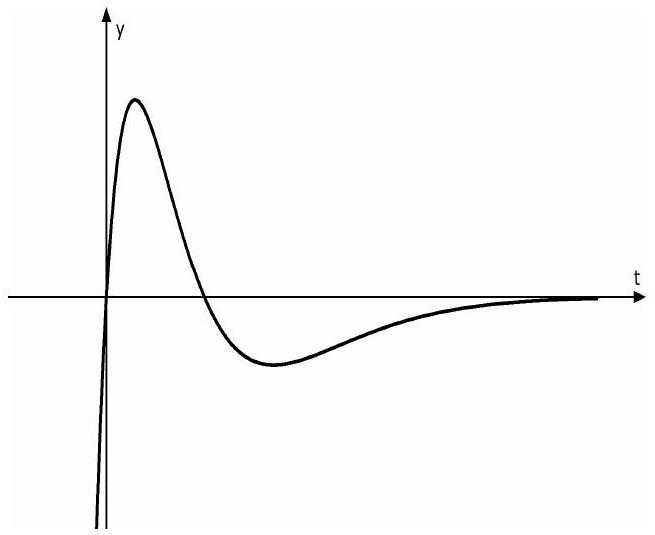
\includegraphics[max width=\textwidth, center]{2025_04_24_473000469cb0f19108adg-2}\\
a) Geben Sie die momentane Änderungsrate des Wasservolumens eine Stunde nach Beobachtungsbeginn an.\\
(0,5 VP)\\
Begründen Sie, dass das Wasservolumen in den ersten beiden Stunden nach Beobachtungsbeginn niemals abnimmt.\\
(1,5 VP)\\
Die momentane Änderungsrate des Wasservolumens besitzt ein Minimum. Bestimmen Sie den Zeitpunkt, zu dem dieses Minimum angenommen wird. (Teilergebnis: $\mathrm{t}_{\min }=2+\sqrt{2}$ )

Die Funktion $F$ mit $F(t)=t^{2} \cdot e^{2-t}$ ist eine Stammfunktion von $f$. Zwei Stunden nach Beobachtungsbeginn enthält das Becken $6 \mathrm{~m}^{3}$ Wasser.\\
b) Ermitteln Sie das Wasservolumen, das sich zu Beobachtungsbeginn im Becken befand.

Es gibt einen 45-Minuten-Zeitraum, in welchem das Wasservolumen um genau einen Kubikmeter zunimmt. Geben Sie eine Gleichung an, deren Lösung den Beginn dieses Zeitraums darstellt.\\
(1 VP)\\
c) Über eine Schaltuhr kann ein Zeitpunkt $t_{0}$ gewählt werden, so dass die momentane Änderungsrate des Wasservolumens nur bis $t_{0}$ durch die Funktion $f$ beschrieben wird und danach konstant auf dem Wert $f\left(\mathrm{t}_{0}\right)$ bleibt.\\
Zeigen Sie, dass $t_{0}$ nicht so gewählt werden kann, dass das Becken sieben Stunden nach Beobachtungsbeginn leer ist.

Für ein anderes Becken beschreiben die Funktion g die momentane Zuflussrate und die Funktion h die momentane Abflussrate des Wassers in Abhängigkeit von der Zeit $t(0 \leq t \leq 17$, $t$ in Stunden nach Beobachtungsbeginn, $g(t)$ und $h(t)$ in Kubikmeter pro Stunde). Die Abbildung zeigt die Graphen der beiden Funktionen g und h.\\
d) Geben Sie den Zeitraum an, in dem das Wasservolumen in diesem Becken abnimmt.

Das abfließende Wasser wird in einem quaderförmigen Tank mit der Grundfläche $12 \mathrm{~m}^{2}$ gesammelt. Dieser ist zu Beobachtungsbeginn leer. Untersuchen Sie, ob das Wasser im Tank höher als 5m steigt.\\
(2 VP)\\
Entscheiden Sie, ob das Becken zu Beobachtungsbeginn leer war, und begründen Sie Ihre Entscheidung.\\
(1,5 VP)\\
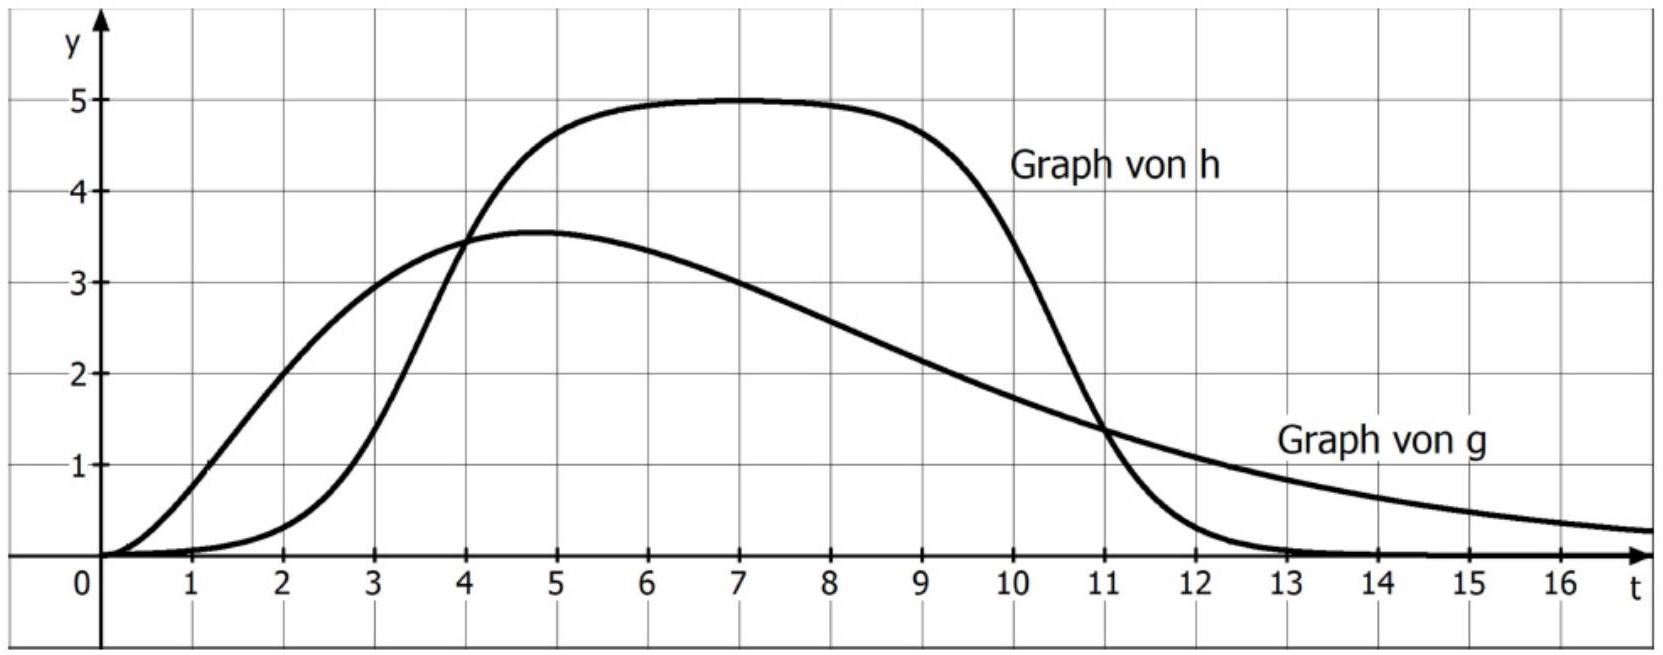
\includegraphics[max width=\textwidth, center]{2025_04_24_473000469cb0f19108adg-3}

\section*{Aufgabe A 2.2 (7 VP)}
Für jede reelle Zahl $a \neq 0$ ist eine Funktion $k_{a}$ gegeben durch $k_{a}(x)=\frac{1}{x}-\frac{a}{x^{2}}$. $G_{a}$ ist der Graph von $k_{a}$.\\
a) Geben Sie Gleichungen der Asymptoten des Graphen $G_{a}$ an.\\
(1 VP)\\
Weisen Sie nach, dass für die Ableitung $k_{a}{ }^{\prime}$ von $k_{a}$ gilt: $k_{a}{ }^{\prime}(x)=\frac{2 a-x}{x^{3}}$\\
(1,5 VP)\\
Zeigen Sie, dass jeder Graph $G_{a}$ genau einen Extrempunkt besitzt, und untersuchen Sie, für welche Werte von a ein Hochpunkt vorliegt.\\
(2,5 VP)\\
b) Jeder Graph $G_{a}$ besitzt einen Punkt $P_{a}$ mit der folgenden Eigenschaft: Die Tangente im Punkt $P_{a}$ an $G_{a}$ verläuft durch den Ursprung.\\
Bestimmen sie die x-Koordinate von $\mathrm{P}_{\mathrm{a}}$.

\section*{Lösungen}
\section*{Aufgabe A 2.1}
a) Geben Sie die momentane Änderungsrate des Wasservolumens eine Stunde nach Beobachtungsbeginn an.\\
$f(t)=\left(2 t-t^{2}\right) \cdot e^{2-t}$\\
$f(1)=1 \cdot e \approx 2,7$ Kubikmeter pro Stunde

Begründen Sie, dass das Wasservolumen in den ersten beiden Stunden nach Beobachtungsbeginn niemals abnimmt.

Nullstellen von $f: f(t)=0$\\
$\left(2 t-t^{2}\right) \cdot \mathrm{e}^{2-t}=0 \quad$ Lösung mit dem Satz vom Nullprodukt\\
I) $2 \mathrm{t}-\mathrm{t}^{2}=0 \Leftrightarrow \mathrm{t} \cdot(2-\mathrm{t})=0$ daraus folgt $\mathrm{t}=0$ oder $\mathrm{t}=2$\\
II) $\mathrm{e}^{2-\mathrm{t}}=0$ ist nicht lösbar

Die einzigen Nullstellen der Funktion $f$ sind $t=0$ und $t=2$.\\
Der Abbildung entnimmt man, dass das Schaubild von f zwischen den Nullstellen oberhalb der t-Achse verläuft, also nimmt das Wasservolumen in den ersten beiden Stunden nie ab.

Die momentane Änderungsrate des Wasservolumens besitzt ein Minimum. Bestimmen Sie den Zeitpunkt, zu dem dieses Minimum angenommen wird.

Notwendige Bedingung: $f^{\prime}(t)=0$\\
$f^{\prime}(\mathrm{t})=(2-2 \mathrm{t}) \cdot \mathrm{e}^{2-\mathrm{t}}+\left(2 \mathrm{t}-\mathrm{t}^{2}\right) \cdot \mathrm{e}^{2-\mathrm{t}} \cdot(-1)=\mathrm{e}^{2-\mathrm{t}} \cdot\left(2-2 \mathrm{t}-2 \mathrm{t}+\mathrm{t}^{2}\right)=\mathrm{e}^{2-\mathrm{t}} \cdot\left(\mathrm{t}^{2}-4 \mathrm{t}+2\right)$ $\mathrm{e}^{2-\mathrm{t}} \cdot\left(\mathrm{t}^{2}-4 \mathrm{t}+2\right)=0$ Lösung mit dem Satz vom Nullprodukt\\
I) $e^{2-t}=0$ ist nicht lösbar\\
II) $\mathrm{t}^{2}-4 \mathrm{t}+2=0 \Rightarrow \mathrm{t}_{1,2}=\frac{4 \pm \sqrt{16-8}}{2}=\frac{4 \pm 2 \sqrt{2}}{2}$

$$
t_{1}=2-\sqrt{2} \approx 0,59 \text { und } t_{2}=2+\sqrt{2} \approx 3,41
$$

Der Abbildung entnimmt man, dass $t_{2}$ die Minimumstelle ist.\\
Etwa 3,4 Stunden nach Beobachtungsbeginn nimmt die Änderungsrate des Wasservolumens ihr Minimum an.\\
b) Ermitteln Sie das Wasservolumen, das sich zu Beobachtungsbeginn im Becken befand.

Das Wasservolumen nach 2 Stunden wird wie folgt berechnet:\\
$V(0)+\int_{0}^{2} f(t) d t=6$\\
$\Leftrightarrow V(0)+F(2)-F(0)=6$\\
Wegen $F(t)=t^{2} \cdot e^{2-t}$ gilt $F(0)=0$ und $F(2)=4$.\\
$\mathrm{V}(0)+4-0=6 \Leftrightarrow \mathrm{~V}(0)=2$\\
Zu Beobachtungsbeginn befanden sich $2 \mathrm{~m}^{3}$ Wasser im Becken.

Geben Sie eine Gleichung an, deren Lösung den Beginn dieses Zeitraums darstellt.

Der 45-Minuten-Zeitraum kann durch das Intervall [t ; $\mathbf{t} \mathbf{+}, 75$ ] dargestellt werden ( t in Stunden).

Bedingung: $\int_{t}^{t+0.75} f(x) d x=1$\\
Auflösung des Integrals ergibt $F(t+0,75)-F(t)=1$\\
Das Wasservolumen wird mithilfe der Stammfunktion $F(t)$ beschrieben.\\
c) Zeigen Sie, dass $t_{0}$ nicht so gewählt werden kann, dass das Becken sieben Stunden nach Beobachtungsbeginn leer ist.

Für den gesuchten Zeitpunkt muss $\mathrm{t}_{0}>2$ gelten, da in den ersten 2 Stunden die momentane Änderungsrate positiv ist.\\
Nach 2 Stunden befinden sich in dem Becken $6 \mathrm{~m}^{3}$ Wasser.\\[0pt]
Wenn das Becken 7 Stunden nach Beobachtungsbeginn leer sein soll, müsste das Wasser im Zeitraum [2;7] mit einer durchschnittlichen oder konstanten Änderungsrate von $-\frac{6 m^{3}}{5 h}=-1,2 \frac{m^{3}}{h}$ abfließen.

Aus b) ergibt sich, dass nach $t_{2}=2+\sqrt{2} \approx 3,41$ Stunden die momentane Abflussrate minimal ist.\\
Diese beträgt $f(2+\sqrt{2}) \approx-1,17 \mathrm{~m}^{3}$ pro Stunde.\\
Da somit die erforderliche Abflussgeschwindigkeit von -1,2 $\mathrm{m}^{3} / \mathrm{h}$ überhaupt nicht erreicht werden kann, kann das Becken nicht nach 7 Stunden leer sein.\\
d) Geben Sie den Zeitraum an, in dem das Wasservolumen in diesem Becken abnimmt.

Das Wasservolumen nimmt ab, solange das Schaubild von h oberhalb des Schaubildes von g liegt.\\
Dies gilt für den Zeitraum 4 Stunden bis 11 Stunden nach Beobachtungsbeginn.

Untersuchen Sie, ob das Wasser im Tank höher als 5m steigt.\\
Wenn das Wasser im Tank eine Höhe von 5 m besitzt, befinden sich $V=12 m^{2} \cdot 5 m=60 m^{3}$ Wasser darin.

Die Menge des abfließenden Wassers entspricht dem Flächeninhalt zwischen dem Schaubild von $h$ und der $t$-Achse.\\
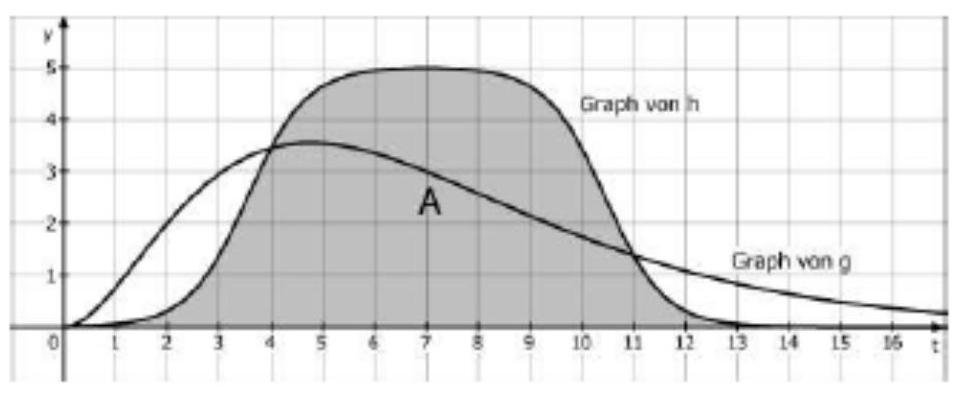
\includegraphics[max width=\textwidth, center]{2025_04_24_473000469cb0f19108adg-6(1)}

1 Kästchen entspricht $1 \mathrm{~m}^{3}$.\\
Da sich zwischen dem Schaubild von $h$ und der t-Achse weniger als 60 Kästchen befinden, steigt das Wasser nicht höher als 5 Meter.

Entscheiden Sie, ob das Becken zu Beobachtungsbeginn leer war, und begründen Sie Ihre Entscheidung.

Der Inhalt der Fläche $A_{1}$ entspricht der Wasserzunahme in dem Becken in den ersten 4 Stunden.\\
Der Inhalt der Fläche $A_{2}$ entspricht der Wasserabnahme in dem Becken zwischen der 4. und 11.Stunde.\\
Da $A_{2}>A_{1}$ ist, kann das Becken zu Beobachtungsbeginn nicht leer gewesen sein.\\
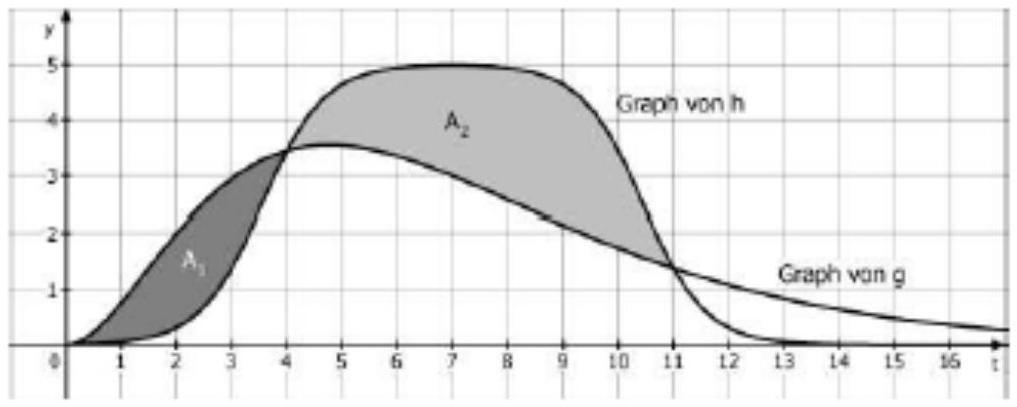
\includegraphics[max width=\textwidth, center]{2025_04_24_473000469cb0f19108adg-6}

\section*{Aufgabe A 2.2:}
a) Geben Sie Gleichungen der Asymptoten des Graphen $\mathrm{G}_{\mathrm{a}}$ an.

$$
k_{a}(x)=\frac{1}{x}-\frac{a}{x^{2}}
$$

Da bei beiden Brüchen der Nennergrad größer als der Zählergrad ist, ist y $=0$ die Gleichung der waagrechten Asymptote.

Da bei $\mathrm{x}=0$ eine Definitionslücke vorliegt, ist $\mathrm{x}=0$ die Gleichung der senkrechten Asymptote.

Weisen Sie nach, dass für die Ableitung $\mathrm{k}_{\mathrm{a}}{ }^{\prime}$ von $\mathrm{k}_{\mathrm{a}}$ gilt: $\mathrm{k}_{\mathrm{a}}{ }^{\prime}(\mathrm{x})=\frac{2 \mathrm{a}-\mathrm{x}}{\mathrm{x}^{3}}$. $\mathrm{k}_{\mathrm{a}}(\mathrm{x})=\frac{1}{\mathrm{x}}-\frac{\mathrm{a}}{\mathrm{x}^{2}}=\mathrm{x}^{-1}-\mathrm{a} \cdot \mathrm{x}^{-2}$\\
$k_{a}^{\prime}(x)=-x^{-2}+2 a \cdot x^{-3}=-\frac{1}{x^{2}}+\frac{2 a}{x^{3}}=-\frac{x}{x^{3}}+\frac{2 a}{x^{3}}=\frac{2 a-x}{x^{3}}$ was zu zeigen war\\
Zeigen Sie, dass jeder Graph $\mathrm{G}_{\mathrm{a}}$ genau einen Extrempunkt besitzt, und untersuchen Sie, für welche Werte von a ein Hochpunkt vorliegt.

Es gilt $\mathrm{k}_{\mathrm{a}}^{\prime \prime}(\mathrm{x})=2 \mathrm{x}^{-3}-6 \mathrm{ax}^{-4}=\frac{2}{\mathrm{x}^{3}}-\frac{6 \mathrm{a}}{\mathrm{x}^{4}}$.\\
Bedingung für Extrempunkt: $\mathrm{k}_{\mathrm{a}}{ }^{\prime}(\mathrm{x})=0$ und $\mathrm{k}_{\mathrm{a}}{ }^{\prime \prime}(\mathrm{x}) \neq 0$\\
$\left.\frac{2 a-x}{x^{3}}=0 \quad \right\rvert\, \cdot x^{3}$\\
$\Leftrightarrow 2 \mathrm{a}-\mathrm{x}=0 \Leftrightarrow \mathrm{x}=2 \mathrm{a}$\\
$k_{a}{ }^{\prime \prime}(2 a)=\frac{2}{(2 a)^{3}}-\frac{6 a}{(2 a)^{4}}=\frac{2}{8 a^{3}}-\frac{6 a}{16 a^{4}}=\frac{1}{4 a^{3}}-\frac{3}{8 a^{3}}=-\frac{1}{8 a^{3}} \neq 0$\\
Somit besitzt jeder Graph $\mathrm{G}_{\mathrm{a}}$ genau einen Extrempunkt.\\
Für einen Hochpunkt muss gelten: $\mathrm{k}_{\mathrm{a}}{ }^{\prime \prime}(2 \mathrm{a})=-\frac{1}{8 \mathrm{a}^{3}}<0$\\
Das ist der Fall für a>0.\\
b) Bestimmen sie die $x$-Koordinate von $\mathrm{P}_{\mathrm{a}}$.

Allgemeine Tangentengleichung an der Stelle $\mathrm{x}=\mathrm{u}$ :\\
$\mathrm{y}=\mathrm{k}_{\mathrm{a}}{ }^{\prime}(\mathrm{u}) \cdot(\mathrm{x}-\mathrm{u})+\mathrm{k}_{\mathrm{a}}(\mathrm{u})$

Einsetzen des Punktes $\mathrm{O}(0 \mid 0)$ : $0=\mathrm{k}_{\mathrm{a}}{ }^{\prime}(\mathrm{u}) \cdot(0-\mathrm{u})+\mathrm{k}_{\mathrm{a}}(\mathrm{u})$

$$
\begin{aligned}
& \left.0=\frac{2 a-u}{u^{3}} \cdot(-u)+\frac{1}{u}-\frac{a}{u^{2}} \right\rvert\, \cdot u^{2} \\
& 0=-2 a+u+u-a \\
& \Leftrightarrow 2 u=3 a \\
& \Leftrightarrow u=\frac{3}{2} a
\end{aligned}
$$

Der Punkt $\mathrm{P}_{\mathrm{a}}$ hat die x -Koordinate $\frac{3}{2} \mathrm{a}$.


\end{document}